\documentclass[12pt]{article}
\usepackage[margin=1.25in]{geometry}
\usepackage{setspace}
\doublespacing


\usepackage{amsmath}
\usepackage{amsfonts}
\usepackage{amsthm}
\usepackage{tikz}
\usepackage[square,numbers]{natbib}
\bibliographystyle{abbrvnat}

\newtheorem{theorem}{Theorem}[section]
\newtheorem{lemma}[theorem]{Lemma}
\newtheorem{corollary}[theorem]{Corollary}
\newtheorem{definition}[theorem]{Definition}

\begin{document}
\title{Burning Spiders}
\author{Ryan DeWolfe}
\date{March 2025}
\maketitle

\abstract{
Burning a graph is a process that models the spread of information in networks.
The process takes place over a discrete number of rounds, and the minimum number of rounds required to burn a graph is the burning number.
The burning number conjecture is that every graph with $n$ vertices has a burning number at most $\lceil \sqrt{n}\ \rceil$.
It has been shown that resolving the burning number conjecture for all graphs is equivalent to resolving it for trees.
A tree is called a spider if it has exactly one vertex with degree strictly greater than $2$.
This work summarizes recent progress by proving the burning number conjecture for spiders.
}

\section{Introduction}
The process of burning a graph was introduced in \cite{burning_intro} to model the spread of information or epidemics.
The burning process take place on graph $G$ and in discrete rounds $t \geq 0$. 
At $t=0$, all the vertices of the graph are unburned.
In each round $t \geq 1$ there are two actions.
First, every burned vertex burns all of its neighbors.
Second, an unburned vertex is selected to be burned.
The process ends when all vertices are burned.

The \textit{burning number} of a graph, denoted $b(G)$, is defined to be the minimum number of rounds required to burn the graph $G$.
We call the sequence of vetices chosen to be burned in action two a \textit{burning sequence}, and the burning number can be equivalently defined as the length of the shortest burning sequence.
Let $n: G \to \mathbb{N}$ be a function counting the number of vertices of $G$, defined as $n(G) = |V(G)|$.
The \textit{burning number conjecture} \cite{burning_intro} is that for all connected graphs, $b(G) \leq \lceil \sqrt{n(G)}\ \rceil$.
This conjecture is currently open, although there has been progress.
We direct the interested reader to the survey \cite{burning_survey} for a general discussion.
Norin and Turcotte \cite{asymptotic_bnc} recently showed that the burning number conjecture hold asymptotically, and the best current bound is $\sqrt{4n(g) \slash 3} + 1$ proved in \cite{best_bnc}. 
It was shown in \cite{burning_intro} that if the burning number conjecture is satisfied in trees, then it is satisfied for all graphs.
Paths acheive the bound $\lceil \sqrt{n}\ \rceil$, showing that if the burning number conjecture would be tight.

This report summarizes the contribution of \cite{burning_spiders} towards the burning number conjecture.
A graph $G$ is a \textit{spider} if it is a connected tree and there is a single vertex with degree strictly greater than two.
The main result is Theorem \ref{thm:main} (Theorem 7 of \cite{burning_spiders}), which confirms that spider graphs satisfy the burning number conjecture. 

\section{Preliminaries}
For this report, we consider all graph to be simple, finite, and undirected.
A \textit{tree} is a graph that does not contain any cycles, a \textit{forest} is a disjoint union of trees, and a \textit{path-forest} is a disjoint union of paths.
Let $G$ be a graph, $v \in V(G)$, and $r$ a positive integer.
Let $N_{r}[v]$ denote the closed neighborhood of $v$ with radius $r$, defined as the set of vertices $u$ such that there is a path from $v$ to $u$ with length less than or equal to $r$.
We let each vertex have a path of length $0$ to itself in order to satisfy the requirements of a metric.
We use $G - N_r[v]$ to represent the graph induced by the set of vertices $V(G) \setminus N_r[v]$. 

\begin{lemma} \label{lem:burntocover}
    A graph $G$ satisfies $b(G) \leq M$ for some integer $M$ if and only if there exists an integer $k$, satisfying $1 \leq k \leq M$, such that
    \begin{equation}
        V(G) = \bigcup_{i = 1}^k N_{M-i}[v_i] \label{eq:burntocover}
    \end{equation}
    for some sequence of vertices $(v_i)_1^k$.
\end{lemma}
\begin{proof}
    Let $G$ be a graph and $(v_i)_1^M$ a burning sequence for $G$.
    Then the fire started at vertex $v_i$ in round $i$ will spread to $N_{M-i}[v_i]$ by the end of round $M$.
    Since $(v_i)_1^M$ burns the graph, let $k = M$ and $V(G) = \cup_{i=1}^M N_{M-i}[v_i]$.
    This concludes the forward implication.

    Let $(v_i)_1^k$ be a sequence in $V(G)$ that satisfies equation \ref{eq:burntocover}.
    Let $(u_j)_1^M$ be a sequence in $V(G)$ where $u_j = v_i$ if $j \leq k$ and the other $u_j$ are any vertex that does not appear earlier in the sequence.
    The fire started at vertex $u_j$ in round $j$ will spread to $N_{M-j}[u_j]$ by round $M$.
    Since $(u_j)_1^M$ burns at least $\cup_{j=1}^M N_{M-j}[u_j] = V(G)$, it is a burning sequnce.
    Thus, $b(G) \leq M$.
\end{proof}

\begin{corollary} \label{cor:leftovers}
    Let $G$ be a graph and $v \in V(G)$.
    Let $\alpha$ be a positive integer.
    If $b(G - N_\alpha[v]) \leq \alpha - 1$, then $b(G) \leq \alpha$.
\end{corollary}
\begin{proof}
    By applying the forward direction of Lemma \ref{lem:burntocover}, there exists some sequence of vertices such that $V(G-N_\alpha[v]) = \cup_{i=1}^{\alpha-1} N_{\alpha-1-i}[v_i]$.
    Let $v_\alpha = v$ and add $N_{\alpha}[v]$ to both sides to get $V(G) = \cup_{i=1}^\alpha N_{\alpha - i}[v_i]$.
    Thus, by the reverse direction of Lemma \ref{lem:burntocover}, $b(G) \leq \alpha$.
\end{proof}

Corollary \ref{cor:leftovers} means that we can bound the burning number of a graph by removing a ``large" neighborhood with radius $\alpha$ and proving the leftovers can be burned in $\alpha - 1$ rounds.
This technique is central to proving many of the following statements.
For proofs the upcoming Lemma \ref{lem:path_forest} and Lemma \ref{lem:family}, we refer to \cite{burning_spiders} (Lemmas 2 and 5 respectively).

\begin{lemma} \label{lem:path_forest}
    If $G$ is a path-forest with $t$ components then $b(G) \leq \lfloor \frac{n(G)}{2t} \rfloor + t$.
\end{lemma}
TODO: double check the $t \geq 1$ condition is just $G$ being non-empty.

%\begin{lemma} \label{lem:path_forest_ceil}
%    If $G$ is a path-forest with $t \leq \sqrt{n(G)}$ components, then $b(G) \leq \lceil \sqrt{n(G)} + \frac{t-1}{2} \rceil$.
%\end{lemma}

\begin{lemma} \label{lem:family}
    Let $\mathcal{G}$ be a set of connected graphs.
    Let $\hat{\mathcal{G}} \subseteq G$ with the following condition.
    For every $G \in \hat{\mathcal{G}}$, there exists $v \in V(G)$ and $r \leq \lceil \sqrt{n(G)}\ \rceil - 1$ such that at least one of the followng conditions are satisfied.
    \begin{enumerate}
        \item $N_r[v] = V(G).$
        \item $|N_r[v]| \geq 2\lceil \sqrt{n(G)}\ \rceil - 1$ and the induced subgraph\\ $G[V(G) \setminus N_r[v]]$ is in  $\mathcal{G}$.
    \end{enumerate}
    If $b(G) \leq \lceil \sqrt{n(G)}\ \rceil$ for all $G \in \mathcal{G} \backslash \hat{\mathcal{G}}$, then $b(G) \leq \lceil \sqrt{n(G)}\ \rceil$ for all $G \in \mathcal{G}$.
\end{lemma}

\section{Spiders}
Recall that a graph $G$ is a spider if it is a connected tree that has a single vertex with degree strictly greater than two.
We call this vertex the \textit{head} of the spider.
An \textit{arm} of a spider is a component of the path forest induced by deleting the head.

\begin{lemma} \label{lem:small_spiders}
    If G is a spider and $n(G) \leq 25$, then $b(G) \leq \lceil \sqrt{n(G)}\ \rceil$.
\end{lemma}
\begin{proof}
    Let $G$ be a spider with head $h$.
    Let $\alpha = \lceil \sqrt{n(G)}\ \rceil$.
    If $\sqrt{n(G)}$ is not an integer, $G$ is an induced graph of a spider $H$ with $n(H) = \alpha^2$.
    If $(v_i)_1^\alpha$ is a burning sequnce for $H$, then $(u_j)_1^\alpha$ is a burning sequence for $G$, where $v_i = u_j$ if $v_i \in V(G)$, and $u_j$ is the closest vertex to $v_i$ that is in $V(G)$ otherwise.
    The chosen vertices are shifted up the arms towards the head, so the neighborhoods that they burn will overlap more, but will still cover the graph.
    Thus, we may assume $n(G)$ is a square integer: $4, 9, 16,$ or $25$.
    
    The unique spider with $n(G) = 4$ is burned in two rounds by choosing the head to burn in round $1$.
    
    Suppose $n(G) = 9$.
    TODO: Why can we assume each arm has length at least $3$? Invoke a path-forest lemma?
    If $G - N_2[h]$ has only one component, the component has length at most $4$ which can be burned in two rounds.
    So, by Corollary \ref{cor:leftovers} $b(G) \leq 3$.
    If $G - N-2[h]$ has two components, the Lemma \ref{lem:path_forest} implies $G-N_2[h]$ can be burned two rounds, and Corollary \ref{cor:leftovers} shows $b(G) \leq 3$.
    Finally, $G -N_2[h]$ cannot have $3$ or more components or else $n(G)$ would be at least $10$.

    Suppose $n(G) = 16$.
    If the head is burned first, every arm with length less than $4$ will be burned by round $4$.
    If an arm is length $7$ or greater, since $2\lceil \sqrt{n(G)}\ \rceil - 1 = 7$, we can burn the end of that arm and apply Lemma \ref{lem:family}.
    The path-forest $G - N_3[h]$ cannot have more than $3$ components or else it would have at least $4 \cdot 4 + 1 = 17$ vertices.
    Since each component of the path-forest $G - N_3[h]$ has at most $3$ vertices, if $G-N_3[h]$ has $1$ or $2$ components then Lemma \ref{lem:path_forest} and Corollary \ref{cor:leftovers} show $b(G) \leq 4$.
    Thus, we must only consider when $G-N_3[h]$ has $3$ components.
    If $G-N_3[h]$ has less than $6$ vertices, apply Lemma \ref{lem:path_forest} and Corollary \ref{cor:leftovers}.
    And there are only two spiders with $3$ arms with lengths between $4$ and $6$ where $n(G-N_3[h]) = 6$.
    Burning sequences are shown in Figure \ref{fig:spiders_n16}.

    \begin{figure}
        \centering
        \begin{tiny}
        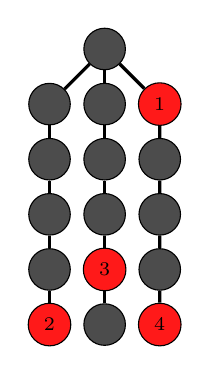
\begin{tikzpicture}[scale=0.7]
            \begin{scope}[every node/.style={fill=black!70,circle,draw=black, minimum size=1.5em}]
                \node[fill=red!90] (1) at (0,0) {\scriptsize 2};
                \node (2) at (1,0) {\:};
                \node[fill=red!90] (3) at (2,0) {\scriptsize 4};

                \node (4) at (0,1) {};
                \node[fill=red!90] (5) at (1,1) {\scriptsize 3};
                \node (6) at (2,1) {};

                \node (7) at (0,2) {};
                \node (8) at (1,2) {};
                \node (9) at (2,2) {};

                \node (10) at (0,3) {};
                \node (11) at (1,3) {};
                \node (12) at (2,3) {};

                \node (13) at (0,4) {};
                \node (14) at (1,4) {};
                \node (15)[fill=red!90] at (2,4) {\scriptsize 1};

                \node (16) at (1,5) {};
            \end{scope}
            \begin{scope}[every edge/.style={draw,very thick}]
                \path [-] (1) edge node {} (4);
                \path [-] (4) edge node {} (7);
                \path [-] (7) edge node {} (10);
                \path [-] (10) edge node {} (13);
                \path [-] (13) edge node {} (16);

                \path [-] (2) edge node {} (5);
                \path [-] (5) edge node {} (8);
                \path [-] (8) edge node {} (11);
                \path [-] (11) edge node {} (14);
                \path [-] (14) edge node {} (16);

                \path [-] (3) edge node {} (6);
                \path [-] (6) edge node {} (9);
                \path [-] (9) edge node {} (12);
                \path [-] (12) edge node {} (15);
                \path [-] (15) edge node {} (16);
            \end{scope}
        \end{tikzpicture}
        \qquad
        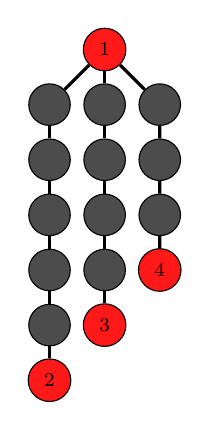
\begin{tikzpicture}[scale=0.7]
            \begin{scope}[every node/.style={fill=black!70,circle,draw=black, minimum size=1.5em}]
                \node (1) at (0,0) {};
                \node[fill=red!90] (2) at (1,0) {\scriptsize 3};
                \node[fill=red!90] (3) at (0,-1) {\scriptsize 2};

                \node (4) at (0,1) {};
                \node (5) at (1,1) {};
                \node[fill=red!90] (6) at (2,1) {\scriptsize 4};

                \node (7) at (0,2) {};
                \node (8) at (1,2) {};
                \node (9) at (2,2) {};

                \node (10) at (0,3) {};
                \node (11) at (1,3) {};
                \node (12) at (2,3) {};

                \node (13) at (0,4) {};
                \node (14) at (1,4) {};
                \node (15) at (2,4) {};

                \node[fill=red!90] (16) at (1,5) {\scriptsize 1};
            \end{scope}
            \begin{scope}[every edge/.style={draw,very thick}]
                \path [-] (1) edge node {} (4);
                \path [-] (4) edge node {} (7);
                \path [-] (7) edge node {} (10);
                \path [-] (10) edge node {} (13);
                \path [-] (13) edge node {} (16);

                \path [-] (2) edge node {} (5);
                \path [-] (5) edge node {} (8);
                \path [-] (8) edge node {} (11);
                \path [-] (11) edge node {} (14);
                \path [-] (14) edge node {} (16);

                \path [-] (3) edge node {} (1);
                \path [-] (6) edge node {} (9);
                \path [-] (9) edge node {} (12);
                \path [-] (12) edge node {} (15);
                \path [-] (15) edge node {} (16);
            \end{scope}
        \end{tikzpicture}
        \end{tiny}
        \caption{
            Burning sequences for the two spiders with $n(G) = 16$ and three arms with lengths at least $4$ and at most $6$.
        }
        \label{fig:spiders_n16}
    \end{figure}

    Suppose $n(G) = 25$.
    We use an analogus argument to $n(G) = 16$.
    If one arm has length greater than $8$, $2 \lceil \sqrt{n(G)} \rceil - 1 = 9$ so Lemma \ref{lem:family} applies with a smaller spider.
    The path-forest $G - N_4[h]$ cannot have more than $4$ components since $5*5 + 1 > n(G)$.
    Since each component of $G-N_4[h]$ has at most $4$ vertices, if $G-N_4[h]$ has only $1$ or $2$ components then Lemma \ref{lem:path_forest} and Corollary \ref{cor:leftovers} apply.
    If $G-N_4[h]$ has $3$ components and less than $12$ vertices, Lemma \ref{lem:path_forest} and Corollary \ref{cor:leftovers} apply.
    And there is only one spider where $G-N_4[h]$ has $3$ components and $n(G-N_4[h]) = 12$.
    If $G-N_4[h]$ has $4$ components and less than $8$ vertices, Lemma \ref{lem:path_forest} and Corollary \ref{cor:leftovers} apply.
    And there are four spiders where $G-N_4[h]$ has $4$ components and $n(G-N_4[h]) = 8$.
    Burning sequences for these spiders are shown in Figure \ref{fig:spiders_n25}.
    
    \begin{figure}
        \begin{tiny}
        \centering
        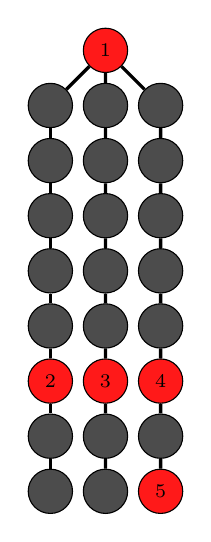
\begin{tikzpicture}[scale=0.7]
            \begin{scope}[every node/.style={fill=black!70,circle,draw=black, minimum size=1.6em}]
                \node (1) at (0,0) {};
                \node (2) at (1,0) {};
                \node[fill=red!90] (3) at (2,0) {\scriptsize 5};

                \node (4) at (0,1) {};
                \node (5) at (1,1) {};
                \node (6) at (2,1) {};

                \node[fill=red!90] (7) at (0,2) {\scriptsize 2};
                \node[fill=red!90] (8) at (1,2) {\scriptsize 3};
                \node[fill=red!90] (9) at (2,2) {\scriptsize 4};

                \node (10) at (0,3) {};
                \node (11) at (1,3) {};
                \node (12) at (2,3) {};

                \node (13) at (0,4) {};
                \node (14) at (1,4) {};
                \node (15) at (2,4) {};

                \node (16) at (0,5) {};
                \node (17) at (1,5) {};
                \node (18) at (2,5) {};

                \node (19) at (0,6) {};
                \node (20) at (1,6) {};
                \node (21) at (2,6) {};

                \node (22) at (0,7) {};
                \node (23) at (1,7) {};
                \node (24) at (2,7) {};

                \node[fill=red!90] (25) at (1,8) {\scriptsize 1};
            \end{scope}
            \begin{scope}[every edge/.style={draw,very thick}]
                \path [-] (1) edge node {} (4);
                \path [-] (4) edge node {} (7);
                \path [-] (7) edge node {} (10);
                \path [-] (10) edge node {} (13);
                \path [-] (13) edge node {} (16);
                \path [-] (16) edge node {} (19);
                \path [-] (19) edge node {} (22);
                \path [-] (22) edge node {} (25);

                \path [-] (2) edge node {} (5);
                \path [-] (5) edge node {} (8);
                \path [-] (8) edge node {} (11);
                \path [-] (11) edge node {} (14);
                \path [-] (14) edge node {} (17);
                \path [-] (17) edge node {} (20);
                \path [-] (20) edge node {} (23);
                \path [-] (23) edge node {} (25);

                \path [-] (3) edge node {} (6);
                \path [-] (6) edge node {} (9);
                \path [-] (9) edge node {} (12);
                \path [-] (12) edge node {} (15);
                \path [-] (15) edge node {} (18);
                \path [-] (18) edge node {} (21);
                \path [-] (21) edge node {} (24);
                \path [-] (24) edge node {} (25);
            \end{scope}
        \end{tikzpicture}
        \hfill
        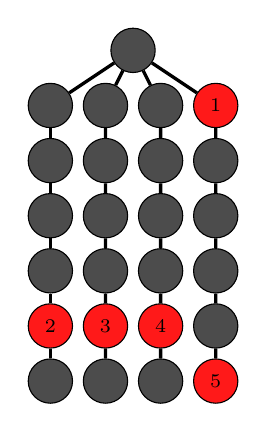
\begin{tikzpicture}[scale=0.7]
            \begin{scope}[every node/.style={fill=black!70,circle,draw=black, minimum size=1.6em}]
                \node (1) at (0,0) {};
                \node (2) at (1,0) {};
                \node (3) at (2,0) {};
                \node[fill=red!90] (4) at (3,0) {\scriptsize 5};

                \node[fill=red!90] (5) at (0,1) {\scriptsize 2};
                \node[fill=red!90] (6) at (1,1) {\scriptsize 3};
                \node[fill=red!90] (7) at (2,1) {\scriptsize 4};
                \node (8) at (3,1) {};

                \node (9) at (0,2) {};
                \node (10) at (1,2) {};
                \node (11) at (2,2) {};
                \node (12) at (3,2) {};

                \node (13) at (0,3) {};
                \node (14) at (1,3) {};
                \node (15) at (2,3) {};
                \node (16) at (3,3) {};

                \node (17) at (0,4) {};
                \node (18) at (1,4) {};
                \node (19) at (2,4) {};
                \node (20) at (3,4) {};

                \node (21) at (0,5) {};
                \node (22) at (1,5) {};
                \node (23) at (2,5) {};
                \node[fill=red!90] (24) at (3,5) {\scriptsize 1};

                \node (25) at (1.5,6) {};
            \end{scope}
            \begin{scope}[every edge/.style={draw,very thick}]
                \path [-] (1) edge node {} (5);
                \path [-] (5) edge node {} (9);
                \path [-] (9) edge node {} (13);
                \path [-] (13) edge node {} (17);
                \path [-] (17) edge node {} (21);
                \path [-] (21) edge node {} (25);

                \path [-] (2) edge node {} (6);
                \path [-] (6) edge node {} (10);
                \path [-] (10) edge node {} (14);
                \path [-] (14) edge node {} (18);
                \path [-] (18) edge node {} (22);
                \path [-] (22) edge node {} (25);

                \path [-] (3) edge node {} (7);
                \path [-] (7) edge node {} (11);
                \path [-] (11) edge node {} (15);
                \path [-] (15) edge node {} (19);
                \path [-] (19) edge node {} (23);
                \path [-] (23) edge node {} (25);

                \path [-] (4) edge node {} (8);
                \path [-] (8) edge node {} (12);
                \path [-] (12) edge node {} (16);
                \path [-] (16) edge node {} (20);
                \path [-] (20) edge node {} (24);
                \path [-] (24) edge node {} (25);
            \end{scope}
        \end{tikzpicture}
        \hfill
        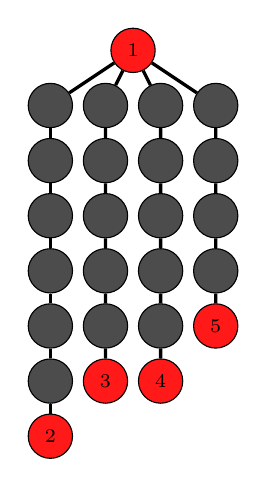
\begin{tikzpicture}[scale=0.7]
            \begin{scope}[every node/.style={fill=black!70,circle,draw=black, minimum size=1.6em}]
                \node (1) at (0,0) {};
                \node[fill=red!90] (2) at (1,0) {\scriptsize 3};
                \node[fill=red!90] (3) at (2,0) {\scriptsize 4};
                \node[fill=red!90] (4) at (0,-1) {\scriptsize 2};

                \node (5) at (0,1) {};
                \node (6) at (1,1) {};
                \node (7) at (2,1) {};
                \node[fill=red!90] (8) at (3,1) {\scriptsize 5};

                \node (9) at (0,2) {};
                \node (10) at (1,2) {};
                \node (11) at (2,2) {};
                \node (12) at (3,2) {};

                \node (13) at (0,3) {};
                \node (14) at (1,3) {};
                \node (15) at (2,3) {};
                \node (16) at (3,3) {};

                \node (17) at (0,4) {};
                \node (18) at (1,4) {};
                \node (19) at (2,4) {};
                \node (20) at (3,4) {};

                \node (21) at (0,5) {};
                \node (22) at (1,5) {};
                \node (23) at (2,5) {};
                \node (24) at (3,5) {};

                \node[fill=red!90] (25) at (1.5,6) {\scriptsize 1};
            \end{scope}
            \begin{scope}[every edge/.style={draw,very thick}]
                \path [-] (1) edge node {} (5);
                \path [-] (5) edge node {} (9);
                \path [-] (9) edge node {} (13);
                \path [-] (13) edge node {} (17);
                \path [-] (17) edge node {} (21);
                \path [-] (21) edge node {} (25);

                \path [-] (2) edge node {} (6);
                \path [-] (6) edge node {} (10);
                \path [-] (10) edge node {} (14);
                \path [-] (14) edge node {} (18);
                \path [-] (18) edge node {} (22);
                \path [-] (22) edge node {} (25);

                \path [-] (3) edge node {} (7);
                \path [-] (7) edge node {} (11);
                \path [-] (11) edge node {} (15);
                \path [-] (15) edge node {} (19);
                \path [-] (19) edge node {} (23);
                \path [-] (23) edge node {} (25);

                \path [-] (4) edge node {} (1);
                \path [-] (8) edge node {} (12);
                \path [-] (12) edge node {} (16);
                \path [-] (16) edge node {} (20);
                \path [-] (20) edge node {} (24);
                \path [-] (24) edge node {} (25);
            \end{scope}
        \end{tikzpicture}
        \hfill
        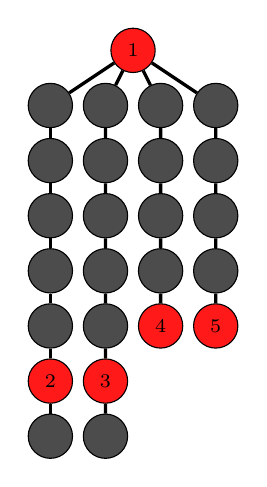
\begin{tikzpicture}[scale=0.7]
            \begin{scope}[every node/.style={fill=black!70,circle,draw=black, minimum size=1.6em}]
                \node[fill=red!90] (1) at (0,0) {\scriptsize 2};
                \node[fill=red!90] (2) at (1,0) {\scriptsize 3};
                \node (3) at (1,-1) {};
                \node (4) at (0,-1) {};

                \node (5) at (0,1) {};
                \node (6) at (1,1) {};
                \node[fill=red!90] (7) at (2,1) {\scriptsize 4};
                \node[fill=red!90] (8) at (3,1) {\scriptsize 5};

                \node (9) at (0,2) {};
                \node (10) at (1,2) {};
                \node (11) at (2,2) {};
                \node (12) at (3,2) {};

                \node (13) at (0,3) {};
                \node (14) at (1,3) {};
                \node (15) at (2,3) {};
                \node (16) at (3,3) {};

                \node (17) at (0,4) {};
                \node (18) at (1,4) {};
                \node (19) at (2,4) {};
                \node (20) at (3,4) {};

                \node (21) at (0,5) {};
                \node (22) at (1,5) {};
                \node (23) at (2,5) {};
                \node (24) at (3,5) {};

                \node[fill=red!90] (25) at (1.5,6) {\scriptsize 1};
            \end{scope}
            \begin{scope}[every edge/.style={draw,very thick}]
                \path [-] (1) edge node {} (5);
                \path [-] (5) edge node {} (9);
                \path [-] (9) edge node {} (13);
                \path [-] (13) edge node {} (17);
                \path [-] (17) edge node {} (21);
                \path [-] (21) edge node {} (25);

                \path [-] (2) edge node {} (6);
                \path [-] (6) edge node {} (10);
                \path [-] (10) edge node {} (14);
                \path [-] (14) edge node {} (18);
                \path [-] (18) edge node {} (22);
                \path [-] (22) edge node {} (25);

                \path [-] (3) edge node {} (2);
                \path [-] (7) edge node {} (11);
                \path [-] (11) edge node {} (15);
                \path [-] (15) edge node {} (19);
                \path [-] (19) edge node {} (23);
                \path [-] (23) edge node {} (25);

                \path [-] (4) edge node {} (1);
                \path [-] (8) edge node {} (12);
                \path [-] (12) edge node {} (16);
                \path [-] (16) edge node {} (20);
                \path [-] (20) edge node {} (24);
                \path [-] (24) edge node {} (25);
            \end{scope}
        \end{tikzpicture}
        \hfill
        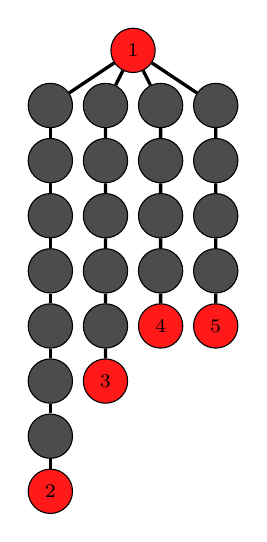
\begin{tikzpicture}[scale=0.7]
            \begin{scope}[every node/.style={fill=black!70,circle,draw=black, minimum size=1.6em}]
                \node (1) at (0,0) {};
                \node[fill=red!90] (2) at (1,0) {\scriptsize 3};
                \node[fill=red!90] (3) at (0,-2) {\scriptsize 2};
                \node (4) at (0,-1) {};

                \node (5) at (0,1) {};
                \node (6) at (1,1) {};
                \node[fill=red!90] (7) at (2,1) {\scriptsize 4};
                \node[fill=red!90] (8) at (3,1) {\scriptsize 5};

                \node (9) at (0,2) {};
                \node (10) at (1,2) {};
                \node (11) at (2,2) {};
                \node (12) at (3,2) {};

                \node (13) at (0,3) {};
                \node (14) at (1,3) {};
                \node (15) at (2,3) {};
                \node (16) at (3,3) {};

                \node (17) at (0,4) {};
                \node (18) at (1,4) {};
                \node (19) at (2,4) {};
                \node (20) at (3,4) {};

                \node (21) at (0,5) {};
                \node (22) at (1,5) {};
                \node (23) at (2,5) {};
                \node (24) at (3,5) {};

                \node[fill=red!90] (25) at (1.5,6) {\scriptsize 1};
            \end{scope}
            \begin{scope}[every edge/.style={draw,very thick}]
                \path [-] (1) edge node {} (5);
                \path [-] (5) edge node {} (9);
                \path [-] (9) edge node {} (13);
                \path [-] (13) edge node {} (17);
                \path [-] (17) edge node {} (21);
                \path [-] (21) edge node {} (25);

                \path [-] (2) edge node {} (6);
                \path [-] (6) edge node {} (10);
                \path [-] (10) edge node {} (14);
                \path [-] (14) edge node {} (18);
                \path [-] (18) edge node {} (22);
                \path [-] (22) edge node {} (25);

                \path [-] (3) edge node {} (4);
                \path [-] (7) edge node {} (11);
                \path [-] (11) edge node {} (15);
                \path [-] (15) edge node {} (19);
                \path [-] (19) edge node {} (23);
                \path [-] (23) edge node {} (25);

                \path [-] (4) edge node {} (1);
                \path [-] (8) edge node {} (12);
                \path [-] (12) edge node {} (16);
                \path [-] (16) edge node {} (20);
                \path [-] (20) edge node {} (24);
                \path [-] (24) edge node {} (25);
            \end{scope}
        \end{tikzpicture}
        \end{tiny}
        \caption{
        Burning sequnces for the five spiders with $n(G) = 25$ and at least 3 arms with length at least $5$ and at most $8$.
        }
        \label{fig:spiders_n25}
    \end{figure}

\end{proof}

\begin{theorem} \label{thm:main}
    If $G$ is a spider then $b(G) \leq \lceil \sqrt{n(G)}\ \rceil$.
\end{theorem}
\begin{proof}
    Let $G$ be a spider.
    If $n(G) \leq 25$, we apply Lemma \ref{lem:small_spiders} and conclude $b(G) \leq \lceil \sqrt{n(G)}\ \rceil$.
    So, suppose $n(G) > 25$ and let $\alpha = \lceil \sqrt{n(G)}\ \rceil$.

    Suppose one arm of $G$ has length $\ell$ and $\ell > 2\alpha - 2$.
    Then for $r = \lceil \frac{\ell}{2} \rceil$ and $v$ the vertex on the arm at a distance $r$ from the head, $|N_r[v]| = 2r + 1 = 2(\lceil \frac{\ell}{2} \rceil) + 1 \geq 2\alpha - 1$ and $G[V(G) \backslash N_r[v]]$ is a spider with one fewer arms.
    TODO: induct on number of arms until either no arms are long or it's only the head. Apply lemma \ref{lem:family} to \{ spiders with long arms \}.
    

    Thus, we must only consider every arm having length at most $2\alpha - 2$.
    
    Suppose $G$ has $\alpha - 1$ arms of length $\alpha + 1$.
    Let $v$ be a vertex adjacent to the head.
    Then $G' = G[V(G) - N_{\alpha - 1}[v]]$ is a path forest with $\alpha - 2$ paths of length $2$ and one path of length $1$.
    By applying Lemma \ref{lem:path_forest} we conclude $b(G') \leq \alpha - 1$ which implies $b(G) \leq \alpha$.

    Suppose otherwise; that is, $G$ does not have $\alpha - 1$ arms of length $\alpha + 1$.
    Let $G' = G[V(G) \backslash N_{\alpha-1}(h)]$ where $h$ is the head of the spider.
    The graph $G'$ is a path forest, and since the arms of $G$ have length at most $2\alpha - 2$, the components of $G'$ have length at most $\alpha - 1$.
    Label the components $G'_1, G'_2, \dotsb , G'_t$ such that $i < j \implies n(G'_i) \leq n(G'_j)$.
    For each $1 \leq i \leq t$, let $v_i$ be a centre of $G'_i$.
    If $t \leq \frac{\alpha}{2}$, then each $G'_i$ is covered by $N_{\alpha - i}[v_i]$, since every $v \in V(G'_i)$ is distance at most $\lfloor \frac{\alpha - 1}{2} \rfloor$ from $v_i$.** 
    Furthermore, if $\alpha$ is odd and $t = \frac{\alpha + 1}{2}$, for each $1 \leq i \leq t-1$ $G'_i$ can be covered by $N_{\alpha-i}[v_i]$ and $G'_{t}$ can be covered by $N_{(\alpha - 1) \slash 2}[v_t] \cup N_{1}[x]$, where $x$ is the end of the path $G'_t$ furtherst from $v_t$.
    Since $\alpha \geq 5$, $\frac{\alpha - 1}{2} > 1$ so these radii are distinct.

    Thus, we need only consider $t \geq \lfloor \frac{\alpha + 1}{2} \rfloor + 1 = \lfloor \frac{\alpha}{2} + \frac{3}{2} \rfloor$. 
    We apply Lemma \ref{lem:path_forest} to show that $b(G') \leq \alpha - 1$.
    Since we removed $\alpha - 1$ vertices from each of the $t$ arms longer than $\alpha - 1$,
    \begin{align}
        n(G') &= n(G) - |N_{\alpha - 1}[h]| \nonumber \\
        &\leq n(G) - \left(t(\alpha - 1) + 1\right) \nonumber \\
        &= \left(\sqrt{n(G)}\right)^2 - 1 - t(\alpha - 1) \nonumber \\
        &= (\sqrt{n(G)} + 1)(\sqrt{n(G)} - 1) - t(\alpha - 1) \nonumber \\
        &\leq (\alpha + 1)(\alpha - 1) - t(\alpha - 1) \nonumber \\
        &= (\alpha - 1)(\alpha + 1 - t) \label{eq:nG}
    \end{align}
    Thus, $t < \alpha + 1$.
    Furthermore, $t \neq \alpha$ since $n(G') \geq t$ and $n(G') \leq \alpha - 1$ (From final line above plugging in $\alpha = t$ into the second bracket).

    Suppose $t = \alpha-1$.
    Applying equation (\ref{eq:nG}) we see $n(G') \leq 2(\alpha-1)$.
    If each of the $t$ components has order $2$, then there were $\alpha - 1$ arms of length $\alpha + 1$, and we have already covered this case.

    So, suppose $\lfloor \frac{\alpha}{2} + \frac{3}{2} \rfloor \leq t \leq \alpha - 2$.
    And 
    \begin{align}
        b(G') &\leq \left\lfloor \frac{n(G)}{2t} \right\rfloor + t \nonumber \\
        &\leq \left\lfloor \frac{(\alpha - 1)(\alpha + 1 - t)}{2t} \right\rfloor + t \nonumber\\
        f(t) &= \left\lfloor \frac{\alpha^2 - 1}{2t} - \frac{\alpha - 1}{2} \right\rfloor + t \label{eq:bupper}
    \end{align}
    Treat equation $\ref{eq:bupper}$ as a real-valued function of $t$ on the domain $t \in [\lfloor \frac{\alpha}{2} + \frac{3}{2} \rfloor, \alpha - 2]$.
    Note that a $t$ maximizing $f(t)$ will also maximise $g(t) = \frac{\alpha^2 - 1}{2t} - \frac{\alpha - 1}{2} + t$.
    However, $g'(t) = -\frac{\alpha^2 - 1}{2t^2} + 1 > 0$ for all $t \in [\lfloor \frac{\alpha}{2} + \frac{3}{2} \rfloor, \alpha - 2]$, so the maximum must be one of the endpoints.

    Let $t = \alpha - 2$ and plug into $\ref{eq:bupper}$, we see
    \begin{align*}
        b(G') &\leq \left\lfloor \frac{(\alpha - 1)(\alpha + 1 - (\alpha - 2))}{2(\alpha - 2)} \right\rfloor + (\alpha - 2)\\
        &= \left\lfloor \frac{\alpha + 1}{2(\alpha - 2)} \right\rfloor + \alpha - 2\\
        &\leq \alpha - 1
    \end{align*}
    With the final inequality due to $\alpha > 5$ and $\frac{\alpha + 1}{2(\alpha - 2)}$ decreasing. 
    
    Let $t = \lfloor \frac{\alpha}{2} + \frac{3}{2}\rfloor$.
    If $\alpha$ is even, then $t = \frac{\alpha}{2} + 1$ and
    \begin{align*}
        b(G') &\leq \left\lfloor \frac{(\alpha - 1)(\alpha + 1 - (\frac{\alpha}{2} + 1))}{2(\frac{\alpha}{2} + 1)} \right\rfloor + (\frac{\alpha}{2} + 1)\\
        &= \left\lfloor \frac{(\alpha - 1)\frac{\alpha}{2}}{\alpha + 2} \right\rfloor + \frac{\alpha}{2} + 1\\
        &= \left\lfloor \frac{(\alpha + 2)\frac{\alpha}{2} - \frac{3\alpha}{2}}{\alpha + 2} \right\rfloor + \frac{\alpha}{2} + 1\\
        &= \left\lfloor \frac{-3\alpha}{2\alpha + 4} \right\rfloor + \alpha + 1\\
        &\leq \alpha - 1
    \end{align*}
    If $\alpha$ is odd, then $t = \frac{\alpha + 1}{2} + 1$ and
    \begin{align*}
        b(G') &\leq \left\lfloor \frac{(\alpha - 1)(\alpha + 1 - (\frac{\alpha + 1}{2} + 1)}{2(\frac{\alpha + 1}{2} + 1)} \right\rfloor + (\frac{\alpha + 1}{2} + 1)\\
        &= \left\lfloor \frac{(\alpha - 1)\frac{\alpha + 1}{2}}{\alpha + 3} \right\rfloor + \frac{\alpha + 1}{2} + 1\\
        &= \left\lfloor \frac{(\alpha + 3)\frac{\alpha + 1}{2} - \frac{4(\alpha + 1)}{2}}{\alpha + 3} \right\rfloor \frac{\alpha + 1}{2} + 1\\
        &= \left\lfloor \frac{-4 (\alpha + 1)}{2\alpha + 6} \right\rfloor \alpha + 2\\
        &\leq \alpha - 1 
    \end{align*}
    Thus, by Corollary \ref{cor:leftovers}, $b(G) \leq \alpha$.
    
\end{proof}

\bibliography{references.bib}

\end{document}